\chapter{Podstawy teoretyczne}
Jak wspomniano w rozdziale~\ref{sec:cele}, dane wejściowe dla programu są wskazaniami pomiarów z~poszczególnych posterunków opadowych. Są to dane punktowe, zatem aby oszacować ilość wody jaka spadła na zadanym obszarze konieczne jest przeprowadzenie ich przekształceniu w~celu wyznaczenia opadu powierzchniowego.

\section{Powrzechne metody wyznaczania opadu powierzchniowego}

Istnieje wiele metod wyznaczania średniego opadu powierzchniowego. Począwszy od prostego obliczenia średniej arytmetycznej wartości z~posterunków opadowych, poprzez metody wieloboków Voronoia, izohiet po hipsometryczną. Różnią się one dokładnością, sposobem aproksymacji czy też zaawansowaniem danych wejściowych~\cite{opad_metody, opad_obliczanie_opadu_sredniego}.

\subsection{Wieloboki Voronoia}
\subsection{Metoda izohiet}
\subsection{Metoda krzywej hipsometrycznej}

\section{Zastosowana metoda}
\label{sec:zastosowana_metoda}
Jak wspomniano we wstępie, praca ta traktuje o analizie danych pojedynczego opadu, a~nie zbieranych przez pewien okres czasu. Przy wyborze sposobu przekształcenia danych jest to bardzo istotne kryterium, które wraz z~możliwością jak najlepszego dopasowania do kształtu zlewni stanowiło główne wymagania tej części pracy. Wybór padł na połączenie techniki triangulacji wraz z~interpolacją przy użyciu płaszczyzny.

\begin{figure}[!ht]
	\centering
	\includegraphics[scale=0.7]{algorytm}
	\caption{Schemat krokowy zastosowanej metody}
	\label{fig:algorytm}
\end{figure}

Triangulacja polega na stworzeniu siatki trójkątów o~wierzchołkach w~zadanych punktach (w tym wypadku są to posterunki opadowe o znanej wysokości opadu). Zastosowano algorytm Delaunay'a, który wprowadza dodatkowe ograniczenie na tworzone trójkąty. Mianowicie, okrąg opisany na każdym z~nich nie może zawierać innych punktów siatki poza wierzchołkami danego trójkąta. Ta metoda ma na celu maksymalizację równoboczności powstałych trójkątów, a~co za tym idzie, równomierność budowanej siatki.

\begin{figure}[!ht]
	\centering
	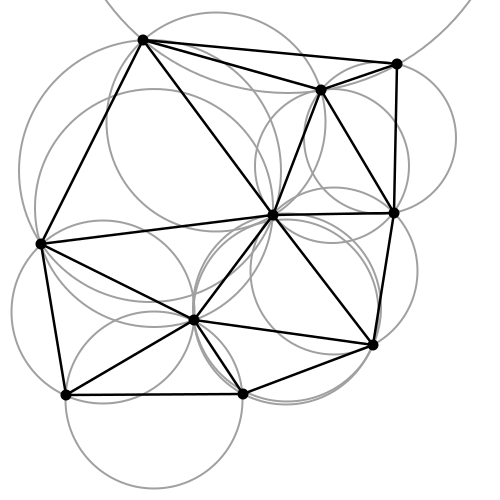
\includegraphics[scale=0.5]{delaunay}
	\caption{Schemat zastosowania algorytmu Delaunay'a (źródło: wikipedia)}
	\label{fig:delaunay}
\end{figure}

Po zastosowaniu triangulacji następnym etapem jest wyznaczenie punktów, dla których należy interpolować wartość opadu. Tymi punktami są poszczególne węzły granicy wskazanej zlewni oraz miejsca przecięcia tej granicy z~krawędziami trójkątów. Wraz z~posterunkami opadowymi znajdującymi się wewnątrz obszaru dla jakiego wyznaczany jest opad powierzchniowy będą stanowiły węzły kolejnej triangulacji.

Wyznaczenie wartości dla wskazanych punktów odbywa się poprzez interpolację płaszczyzną przechodzącą przez trzy punkty (będące wierzchołkami kolejnych trójkątów). Ustalane są współrzędne wektorów normalnych dla poszczególnych płaszczyzn (czyli wektorów prostopadłych do powierzchni danej płaszczyzny), a~następnie korzystając ze wzoru~\ref{eq:wartosc_interpolowana}, wyznaczana jest wartość opadu ($z$) w~punkcie o~zadanych współrzędnych~$x$~i~$y$.

Równanie płaszczyzny przedstawia się następująco

\begin{equation}
\begin{gathered}
A(x - x_0) + B(y - y_0) + C(z - z_0) = 0 \\
[A, B, C] = (P_2 - P_1) \times (P_3 - P_2)
\label{eq:rownanie_plaszczyzny}
\end{gathered}
\end{equation}
gdzie
% eqwhere z aghdpl powoduje błąd
\begin{description}[leftmargin=3cm, itemsep=0cm, labelsep=0cm]
	\item[$x_0, y_0, z_0$] współrzędne punktu należącego do płaszczyzny,
	\item[$A, B, C$] wektor normalny płaszczyzny, %rozwiązać problem z [ ] jako wektor
	\item[$A, B, C$] nie mogą być jednocześnie równe 0.
\end{description}
%
Co po przekształceniu daje
\begin{equation}
\label{eq:wartosc_interpolowana}
	z = \frac{A(x - x_0) + B(y - y_0)}{-C} + z_0
\end{equation}
gdzie $C \neq 0$.


Jeżeli $C$, ze wzoru~\ref{eq:wartosc_interpolowana}, przyjmuje wartość 0 oznacza to, iż w~każdym wierzchołku trójkąta opad był zerowy. Wówczas punktowi interpolowanemu przypisuje się takowe wskazanie.

Po przeprowadzeniu interpolacji wartości dokonuje się ponownej triangulacja, tym razem z~użyciem punktów interpolowanych oraz posterunków wewnątrz zlewni. Nowopowstała siatka trójkątów, wraz z~trzecim wymiarem jakim jest wysokość opadu, tworzy zbiór brył o~trójkątnych podstawach. Wyznaczając i~sumując objętość opadu w~każdej z~nich uzyskiwany jest łączny opad na wskazanej zlewni~\cite{matematyka_poradnik, mathMonthly}.

\begin{equation}
\label{eq:opad_powierzchniowy}
	V = \sum_{i=1}^{n}P_{pi}*\frac{h_{i1}+h_{i2}+h_{i3}}{3}
\end{equation}
gdzie
\begin{description}[leftmargin=3cm, itemsep=0cm, labelsep=0cm]
	\item[$V$] łączna objętość opadu,
	\item[$n$] ilość wyznaczonych brył,
	\item[$P_{pi}$] pole podstawy i-tej bryły,
	\item[$h_{i1}, h_{i2}, h_{i3}$] długość krawędzi bocznej bryły (wartość opadu) w~danym wierzchołku.
\end{description}




\section{Możliwe rozszerzenia algorytmu}
Oczywiście można dążyć do usprawnienia metody przekształcania danych wejściowych.
Przykładowe rozszerzenia mogą obejmować
\begin{itemize}
\item{ Analizę sąsiednich dla trójkąta punktów i~na ich podstawie wyznaczyć wartość opadu w~środku zadanego fragmentu, a~dalej dzielić go na mniejsze. }
\item{ Interpolacja powierzchnią inną niż płaszczyzna. Kształt powierzchni definiować na bazie większej ilościu punktów znanych. }
\end{itemize}